% =============================================================================
% COPYRIGHT AND DISCLAIMER
% =============================================================================
% This file is provided as a convenience template for competition participants.
% By using it, you accept full responsibility for compliance with all applicable
% copyright, licensing, and usage rules of the Association for Computing
% Machinery (ACM) and of any LaTeX packages you load (including, without
% limitation, the "acmart" document class and related ACM materials).
%
% Consult ACM's official publication, template, and copyright policies before
% using this setup for any purpose other than this competition. Do not assume
% that this template may be reused, redistributed, or submitted elsewhere
% without independently verifying ACM's current rules.
%
% Use of the "acmart" class, the "sigconf" option, or ACM-style formatting in
% this template does NOT mean that this report, this competition, its organizers,
% or any resulting PDF is sponsored, endorsed, affiliated with, or published by
% ACM. ACM trademarks and branding remain the property of ACM.
%
% Template packages live in preamble.tex.
% Citations live in main.bib. Edit this file with your paper content.
% =============================================================================

\documentclass[sigconf]{acmart}
% =============================================================================
% Template setup — participants normally do not edit this file.
% Author content belongs in main.tex; citations belong in main.bib.
% \documentclass lives in main.tex so Overleaf does not treat this file as root.
% =============================================================================

% --- Competition / non-ACM-submission friendly rights metadata -------------
\setcopyright{none}
\settopmatter{printacmref=false}
\acmConference[Kaggle Competition]{Filament Segmentation Challenge}{2026}{\href{https://www.kaggle.com/competitions/filament-segmentation-2026}{kaggle.com/competitions/filament-segmentation-2026}}
\acmBooktitle{Competition Report}
\acmDOI{}
\acmISBN{}

% --- Author guidance text --------------------------------------------------
% \guide{...} is gray italic while \guideStyletrue; omitted from the PDF if false.
% Flip the switch in main.tex after % =============================================================================
% Template setup — participants normally do not edit this file.
% Author content belongs in main.tex; citations belong in main.bib.
% \documentclass lives in main.tex so Overleaf does not treat this file as root.
% =============================================================================

% --- Competition / non-ACM-submission friendly rights metadata -------------
\setcopyright{none}
\settopmatter{printacmref=false}
\acmConference[Kaggle Competition]{Filament Segmentation Challenge}{2026}{\href{https://www.kaggle.com/competitions/filament-segmentation-2026}{kaggle.com/competitions/filament-segmentation-2026}}
\acmBooktitle{Competition Report}
\acmDOI{}
\acmISBN{}

% --- Author guidance text --------------------------------------------------
% \guide{...} is gray italic while \guideStyletrue; omitted from the PDF if false.
% Flip the switch in main.tex after % =============================================================================
% Template setup — participants normally do not edit this file.
% Author content belongs in main.tex; citations belong in main.bib.
% \documentclass lives in main.tex so Overleaf does not treat this file as root.
% =============================================================================

% --- Competition / non-ACM-submission friendly rights metadata -------------
\setcopyright{none}
\settopmatter{printacmref=false}
\acmConference[Kaggle Competition]{Filament Segmentation Challenge}{2026}{\href{https://www.kaggle.com/competitions/filament-segmentation-2026}{kaggle.com/competitions/filament-segmentation-2026}}
\acmBooktitle{Competition Report}
\acmDOI{}
\acmISBN{}

% --- Author guidance text --------------------------------------------------
% \guide{...} is gray italic while \guideStyletrue; omitted from the PDF if false.
% Flip the switch in main.tex after \input{preamble}.
%
% Do not use \guide{...} for \email{...}.
\usepackage{xcolor}
\newif\ifguideStyle
\guideStyletrue
\newcommand{\guide}[1]{%
  \ifguideStyle
    {\color{gray!65}\itshape #1}%
  \fi
}

% --- Math ------------------------------------------------------------------
% Do NOT load amssymb (or amsfonts): acmart already loads newtxmath, which
% defines the same symbols (e.g. \Bbbk) and causes a conflict on Overleaf.
% amsmath is already provided by acmart; mathtools extends it.
\usepackage{mathtools}

% --- Figures ---------------------------------------------------------------
% graphicx is already loaded by acmart
\usepackage{subcaption}

% --- Tables ----------------------------------------------------------------
% booktabs is already loaded by acmart
\usepackage{tabularx}
\usepackage{multirow}

% --- Bibliography style is set in main.tex (ACM-Reference-Format) ----------
.
%
% Do not use \guide{...} for \email{...}.
\usepackage{xcolor}
\newif\ifguideStyle
\guideStyletrue
\newcommand{\guide}[1]{%
  \ifguideStyle
    {\color{gray!65}\itshape #1}%
  \fi
}

% --- Math ------------------------------------------------------------------
% Do NOT load amssymb (or amsfonts): acmart already loads newtxmath, which
% defines the same symbols (e.g. \Bbbk) and causes a conflict on Overleaf.
% amsmath is already provided by acmart; mathtools extends it.
\usepackage{mathtools}

% --- Figures ---------------------------------------------------------------
% graphicx is already loaded by acmart
\usepackage{subcaption}

% --- Tables ----------------------------------------------------------------
% booktabs is already loaded by acmart
\usepackage{tabularx}
\usepackage{multirow}

% --- Bibliography style is set in main.tex (ACM-Reference-Format) ----------
.
%
% Do not use \guide{...} for \email{...}.
\usepackage{xcolor}
\newif\ifguideStyle
\guideStyletrue
\newcommand{\guide}[1]{%
  \ifguideStyle
    {\color{gray!65}\itshape #1}%
  \fi
}

% --- Math ------------------------------------------------------------------
% Do NOT load amssymb (or amsfonts): acmart already loads newtxmath, which
% defines the same symbols (e.g. \Bbbk) and causes a conflict on Overleaf.
% amsmath is already provided by acmart; mathtools extends it.
\usepackage{mathtools}

% --- Figures ---------------------------------------------------------------
% graphicx is already loaded by acmart
\usepackage{subcaption}

% --- Tables ----------------------------------------------------------------
% booktabs is already loaded by acmart
\usepackage{tabularx}
\usepackage{multirow}

% --- Bibliography style is set in main.tex (ACM-Reference-Format) ----------


% Pipeline diagram (Figure 1)
\usepackage{tikz}
\usetikzlibrary{positioning,arrows.meta}

% Guide styling: \guideStyletrue = show gray italic hints; \guideStylefalse = omit them
% \guideStyletrue
\guideStylefalse

\newcommand{\repourl}{\url{https://github.com/ii56/Solar-Filament-Segmentation-Challenge-2026}}

\begin{document}

\title{Tiled U-Net Segmentation with Hysteresis-Based Instance Extraction}  % Replace this with your title
\subtitle{A Solution to the Solar Filament Segmentation Challenge 2026} % DO NOT CHANGE


\author{Ibaan Ibrahim}
\affiliation{%
  \institution{Asia Pacific University of Technology \& Innovation}
  \city{Kuala Lumpur}
  \country{Malaysia}
}
\email{ibaanibrahim123098@gmail.com}

\begin{abstract}
    This report describes our solution to the Solar Filament Segmentation Challenge~2026, a Kaggle competition on automatic segmentation of solar filaments in GONG H-$\alpha$ observations. I train a class-agnostic U-Net with an ImageNet-pretrained ResNet-34 encoder on contrast-equalised $512\times512$ tiles, using binary cross-entropy plus a Tversky loss, and stitch the tile outputs into a full-disk probability map. Instances are then extracted with hysteresis thresholding, where a connected region is kept only if its peak probability reaches a high threshold. This removed most of my false detections and left the masks themselves almost unchanged. On a held-out half of my validation photos the method reaches a Panoptic Quality (PQ) of $0.361\pm0.017$ and a foreground Dice of $0.62$. For comparison, two annotators labelling the same photo agree with each other at PQ $0.37$. Inference takes 0.85\,s per image on a 4\,GB laptop GPU.
\end{abstract}

\maketitle

\ifguideStyle
\noindent{\color{gray!65}\itshape
Guide mode is on.}
\par\medskip
\fi

\guide{Please limit your report to four (4) pages, excluding the Acknowledgment and References sections. Throughout this document, please follow these considerations:
\begin{itemize}
    \item Do not alter any text that is currently in black color (except for the emails under authors' name).
    \item Replace all gray text with your own.
    \item When you are done with the report, please replace \texttt{\textbackslash guideStyletrue} with \texttt{\textbackslash guideStylefalse}, to remove any gray text. Alternatively, you can remove any text wrapped in \texttt{\textbackslash guide\{\}},
    \item Be as succinct as possible, and only provide details regarding your own work. For example, there is no need to discuss what solar filaments are, or why filament segmentation matters.
    \item If you must, you can add extra sections.
\end{itemize}}


% ==================================== %
%              INTRODUCTION            %
% ==================================== %
\section{Introduction}
    This report goes over the details of our submitted solution to the Solar Filament Segmentation Challenge~2026 \cite{filament-segmentation-2026}. The challenge, launched on July~10,~2026, is organized by the Earth-Space AI Research (ESAIR) Lab\footnote{\href{https://www.esairlab.com/home}{www.esairlab.com/}}. This challenge utilizes the MAGFiLO dataset for evaluation of the segmentation algorithms \cite{ahmadzadeh2024dataset}.
    Submissions are scored by Panoptic Quality (PQ) \cite{kirillov2019panoptic}, so each filament has to be predicted as a separate mask. I handle this in two steps: a semantic segmentation network predicts a filament probability for every pixel, and a post-processing step turns that map into instances. My first PQ measurements showed that false detections were costing me much more than mask quality was, so a large part of the work went into the instance extraction step. I chose its rule by looking at statistics of the predicted regions, and I tuned and reported on separate sets of photos. Everything was trained and run on one laptop GPU with 4\,GB of memory. The code, with a notebook that reproduces the submission, is at \repourl.


% ==================================== %
%              METHODOLOGY             %
% ==================================== %
\section{Methodology}\label{sec:methodology}

\begin{figure*}[t]
\centering
\begin{tikzpicture}[
    box/.style={draw, rounded corners=2pt, align=center, font=\scriptsize,
                text width=1.92cm, minimum height=1.05cm, inner sep=2pt, fill=#1},
    box/.default=white,
    arr/.style={-{Stealth[length=4pt]}, thick},
    node distance=0.32cm]
  % inference path
  \node[box=blue!6]   (img)  {H-$\alpha$ image\\$2048\times2048$, grey};
  \node[box=blue!6, right=of img]  (cl)   {CLAHE\\clip 1.0, $16\times16$ grid};
  \node[box=blue!6, right=of cl]   (tile) {25 tiles $512^2$\\stride 384\\(128 px overlap)};
  \node[box=orange!15, right=of tile] (net) {U-Net\\ResNet-34 encoder\\24.4\,M params};
  \node[box=blue!6, right=of net]  (avg)  {sigmoid; average\\overlapping tiles\\$\to$ probability map};
  \node[box=green!10, right=of avg] (hys) {hysteresis: region\\$p>0.4$, kept if\\$\max p\ge0.995$, area $\ge400$};
  \node[box=blue!6, right=of hys]  (out)  {connected regions\\= instances\\$\to$ COCO RLE (CSV)};
  \foreach \a/\b in {img/cl, cl/tile, tile/net, net/avg, avg/hys, hys/out} \draw[arr] (\a) -- (\b);
  % training path
  \node[box=gray!8, below=0.55cm of img]  (poly) {COCO polygons\\(class labels\\ignored)};
  \node[box=gray!8, right=of poly] (clip) {clip to tile\\(shapely), rasterise\\(pycocotools)};
  \node[box=gray!8, right=of clip] (drop) {drop 50\% of\\empty tiles\\$\to$ 17{,}442 tiles};
  \node[box=gray!8, right=of drop] (loss) {BCE + Tversky\\Adam, AMP\\batch 4, cosine LR};
  \node[font=\scriptsize, align=left, right=0.25cm of loss, text width=5.5cm] (note)
       {\textbf{Training} (grey) shares the CLAHE and tiling\\of the inference path (blue). Split by photo:\\601 train / 106 val photos; val halves A (tune) / B (report).};
  \foreach \a/\b in {poly/clip, clip/drop, drop/loss} \draw[arr] (\a) -- (\b);
  \draw[arr, dashed] (loss) -- node[right, font=\scriptsize]{weights} (net);
\end{tikzpicture}
\caption{End-to-end pipeline. Inference (top) and training (bottom) share the same pre-processing. All settings shown are those used for the submission.}
\label{fig:pipeline}
\Description{Flow diagram of the inference and training pipelines.}
\end{figure*}

\subsection{Data and sampling}
The training set has 1{,}154 annotation entries covering 707 distinct photos and 8{,}199 filament polygons. 296 of the photos were labelled by more than one annotator, so the same photo can appear under several image ids. I therefore split by photo and never by image id, since splitting by id would put the same pixels in both training and validation. 15\% of the photos (seed 42) are held out for validation, giving 601 photos (993 entries) for training and 106 photos (161 entries) for validation. Validation is split again by photo into half A (53 photos, 77 entries) and half B (53 photos, 84 entries). I tuned post-processing on A and used B only for reporting. The chirality classes are ignored because scoring uses the masks only, so the model is class-agnostic.

\subsection{Pre-processing and tiling}
Images are read as greyscale and contrast-equalised with CLAHE \cite{zuiderveld1994clahe} (clip limit 1.0, $16\times16$ grid). I picked these settings by eye; higher clip limits and coarser grids made the chromospheric granulation look like noise. Each $2048\times2048$ image is cut into 25 tiles of $512\times512$ with stride 384. At this size, 97.5\% of the filament bounding boxes fit within 80\% of a tile. The polygons (all parts, for filaments stored in several pieces) are repaired if invalid, clipped to each tile with shapely and rasterised with pycocotools. Many tiles contain no filament at all, so I randomly drop half of those from the training set, leaving 17{,}442 training tiles. All 4{,}025 validation tiles are kept. I did not use any data augmentation.

\subsection{Model and loss}
The network is a U-Net \cite{ronneberger2015unet} with a ResNet-34 encoder \cite{he2016resnet} pretrained on ImageNet \cite{deng2009imagenet}, built with \texttt{segmentation\_models\_pytorch} \cite{iakubovskii2019smp}. It takes one input channel and outputs one logit per pixel (24.4\,M parameters). The loss is
\begin{equation}
\mathcal{L} = \mathrm{BCE}(z, y) + \Bigl(1 - \tfrac{TP + s}{TP + \alpha FP + \beta FN + s}\Bigr),
\end{equation}
i.e.\ binary cross-entropy plus the Tversky loss \cite{salehi2017tversky}, with soft counts from $\sigma(z)$, $\alpha=0.3$, $\beta=0.7$ and $s=1$. With $\beta>\alpha$, a missed filament pixel costs more than a spurious one. My first attempt used Tversky alone, and the model collapsed to predicting background everywhere. On an empty tile, predicting nothing brings that loss to zero, and once the logits saturate its gradient (which has a $\sigma(1-\sigma)$ factor) disappears. Adding BCE keeps a usable gradient on missed positives. I compute the loss in float32 even under mixed precision, since the soft counts can overflow float16.

\subsection{Training}
I train with Adam \cite{kingma2015adam} (learning rate $10^{-4}$, batch size 4, automatic mixed precision). One epoch takes about 27 minutes on an NVIDIA RTX~2050 (4\,GB). With a constant learning rate, validation IoU jumped around between 0.30 and 0.45 from epoch to epoch and never settled (Figure~\ref{fig:curves}), so I restarted from the best constant-rate weights (epoch 12) and trained 10 more epochs with cosine decay \cite{loshchilov2017sgdr} from $10^{-4}$ to $10^{-6}$. I select checkpoints by mean validation IoU over the tiles that contain filaments. Validation loss turned out to be misleading here: about 60\% of validation tiles are empty, so a model that predicts nothing gets a low loss. The submitted model is epoch 8 of the cosine stage, after roughly 9 GPU-hours of training in total.

\begin{figure}[t]
\centering
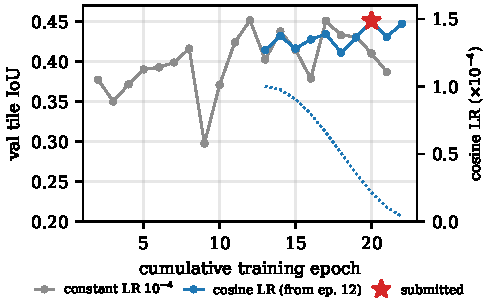
\includegraphics[width=\columnwidth]{figures/curves.pdf}
\caption{Validation tile IoU during training. The constant-rate run is in grey; the cosine stage (blue, learning rate dotted) starts from the epoch-12 weights.}
\label{fig:curves}
\Description{Validation IoU against training epoch for the two training stages.}
\end{figure}

\subsection{Inference and instance extraction}
At test time each image goes through the same CLAHE and tiling. The 25 tiles are run in batches of 8 and the sigmoid outputs are averaged where tiles overlap. I average because taking the maximum favoured whichever tile happened to see a filament closest to its centre. The result is a $2048\times2048$ probability map $p$.

An instance is a connected region of $p>\tau_{\text{low}}$ that passes two checks: its peak probability reaches $\tau_{\text{high}}$, and its area is at least $A_{\min}$ pixels. This is hysteresis thresholding \cite{canny1986edge} applied to whole regions. The low threshold decides how far a region extends and the high threshold decides whether it is kept. I arrived at this rule by recording, for every predicted region on the validation set, its area, mean and peak probability, elongation, and whether it matched a real filament. Regions whose peak stayed below about 0.99 matched a filament only about 2\% of the time, yet they made up 44\% of all false positives. Shape separated the two groups much less well than peak probability did. The submitted setting, chosen on half A, is $\tau_{\text{low}}=0.4$, $\tau_{\text{high}}=0.995$ and $A_{\min}=400$\,px.

I also tried morphological closing with radii of 2 to 10\,px to rejoin broken filaments (the larger radii merged neighbouring filaments instead), minimum elongation and mean-probability filters, a fallback region for images with no detection, and averaging the weights of several checkpoints. None of these improved validation PQ, so none are used. Each instance is written as a COCO run-length encoding, and I decode every row of the submission file again and compare it pixel by pixel with its instance map. The test submission has 1{,}442 instances over 177 of the 180 test images. Figure~\ref{fig:examples} shows some examples.

\begin{figure*}[t]
\centering
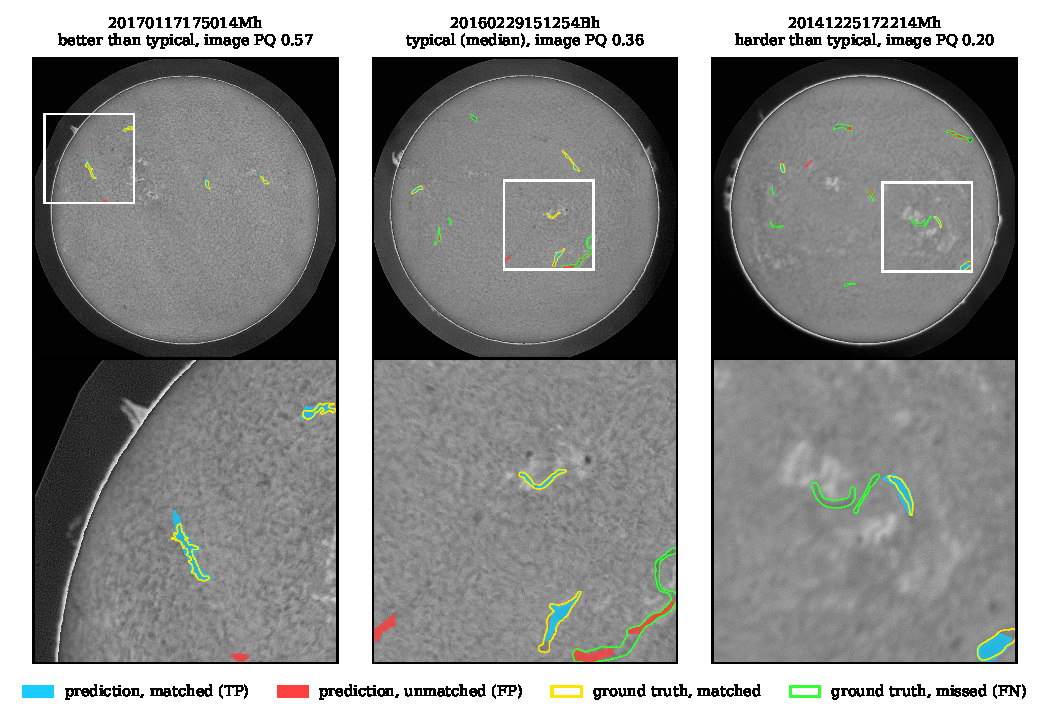
\includegraphics[width=0.9\textwidth]{figures/examples.pdf}
\caption{Predictions on held-out validation photos (half B) at the 90th, 50th and 12th percentile of per-image PQ. Top row: full disk. Bottom row: the boxed $600\times600$ region at full resolution. Predictions are filled and ground truth is outlined.}
\label{fig:examples}
\Description{Three solar disk images with predicted and ground-truth filaments overlaid, plus zoomed crops.}
\end{figure*}


% ==================================== %
%              EVALUATION              %
% ==================================== %
\section{Evaluation}\label{sec:evaluation}

\subsection{Strategy}
I score with PQ = $\sum_{\mathrm{TP}}\mathrm{IoU} / (|\mathrm{TP}| + \frac12|\mathrm{FP}| + \frac12|\mathrm{FN}|)$, where a prediction and a ground-truth filament match when their IoU exceeds 0.5. PQ is the product of segmentation quality (SQ, the mean IoU of the matches) and recognition quality (RQ, an F1 score over instances). Counts are pooled over all images, and each annotator's version of a photo counts as a separate image. Running the PQ code from the organisers' self-evaluation notebook on my validation predictions gave exactly the same numbers as my own implementation. I also report foreground Dice: all filament pixels of an image merged into one mask, then averaged over images. For uncertainty I bootstrap over photos (2{,}000 resamples with replacement, all annotator versions of a photo kept together) and give the standard deviation and the 95\% interval. All settings were fixed on half A, so the half-B numbers are my estimates.

\subsection{Results}
Table~\ref{tab:postproc} compares instance extraction rules on the submitted network. Thresholding at 0.5 with no filter gives PQ 0.275 on B, with 614 false regions against 299 matches. Hysteresis removes more than half of those false regions without losing a single match, and RQ goes from 0.42 to 0.55. SQ (0.65) and Dice (about 0.62) hardly change, so the improvement comes almost entirely from recognition. A plain area filter comes close on B, but it loses some matches (208 missed filaments become 232). On half A it is 0.04 below hysteresis, while on B the difference is only 0.003. I take this as a sign that gaps measured on the tuning half are inflated.

\begin{table}[t]
\caption{Instance extraction on the submitted network. PQ on the tuning half A and on the held-out half B (bootstrap s.d.). SQ, RQ, FP, FN and Dice are on B.}
\label{tab:postproc}
\small
\setlength{\tabcolsep}{3pt}
\begin{tabular}{@{}lcccccc@{}}
\toprule
Rule & PQ$_A$ & PQ$_B$ & SQ & RQ & FP / FN & Dice \\
\midrule
$p>0.5$, no filter          & .295 & .275{\scriptsize$\pm$.018} & .653 & .421 & 614 / 208 & .617 \\
$p>0.5$, area $\ge20$       & .318 & .297{\scriptsize$\pm$.018} & .653 & .454 & 510 / 208 & .617 \\
$p>0.3$, area $\ge800$      & .350 & .358{\scriptsize$\pm$.018} & .648 & .552 & 215 / 232 & .614 \\
hysteresis, area $\ge20$    & .378 & .358{\scriptsize$\pm$.017} & .650 & .550 & 294 / 203 & .625 \\
\textbf{hysteresis, area $\ge400$} & \textbf{.388} & \textbf{.361}{\scriptsize$\pm$.017} & .651 & .554 & 274 / 208 & .623 \\
\bottomrule
\end{tabular}
\end{table}

\begin{table}[t]
\caption{Checkpoints with the submitted post-processing. Annotator agreement: one annotator's labels scored against another's on the 36 validation photos with several annotators (74 pairs).}
\label{tab:models}
\small
\setlength{\tabcolsep}{4pt}
\begin{tabular}{@{}lccc@{}}
\toprule
 & PQ$_A$ & PQ$_B$ & Dice$_B$ \\
\midrule
Constant LR, epoch 12        & .351 & .334{\scriptsize$\pm$.017} & .593 \\
Cosine, epoch 8 (\textbf{submitted}) & .388 & .361{\scriptsize$\pm$.017} & .623 \\
Cosine, epoch 10 (last)      & .370 & .339{\scriptsize$\pm$.015} & .613 \\
\midrule
 & \multicolumn{3}{c}{PQ / SQ / RQ on multi-annotator photos} \\
Annotator vs.\ annotator     & \multicolumn{3}{c}{.366 / .638 / .573} \\
Model vs.\ each annotator    & \multicolumn{3}{c}{.385 / .655 / .588} \\
\bottomrule
\end{tabular}
\end{table}

Table~\ref{tab:models} compares checkpoints. The cosine stage adds 0.027 PQ on B over the constant-rate model. The last cosine epoch, which I did not select, scores 0.339, so some of the selected checkpoint's lead is luck in the selection. Allowing for that, I expect a PQ of roughly 0.34 to 0.36 (the 95\% interval on B is 0.328 to 0.394). Results are similar across the six GONG sites, with per-site validation PQ between 0.359 and 0.389.

The lower part of Table~\ref{tab:models} gives a human reference. On photos labelled by more than one annotator, the annotators agree with each other at PQ 0.366, and their SQ (0.638) is no higher than the model's. I think much of the remaining gap comes from genuine ambiguity in the labels, such as where a filament ends or whether a faint one is there at all. The model scores 0.385 on the same photos, but some of them are in the tuning half, so I would only call this comparable to human agreement.

The public leaderboard shows a mean Dice score on about half of the test images, and my submission scored 0.29 there. This is not the foreground Dice in Table~\ref{tab:postproc}. The organisers' evaluation code computes Dice between individual filaments, and if every matched pair (IoU~$>0.5$) contributes its Dice and every false or missed filament contributes 0, my validation predictions score 0.31 (0.307 averaged per image). Pooled over all pixels per image instead, they score 0.61. The exact leaderboard formula is not published, but the instance-level reading fits the leaderboard well. The test predictions also look very similar to the validation predictions in instances per image (8.0 and 7.4), median instance area (1{,}390 and 1{,}415\,px) and foreground fraction.

On the RTX~2050, inference takes 0.85\,s per $2048\times2048$ test image: 0.04\,s to read the image and apply CLAHE, 0.49\,s for the network on 25 tiles, 0.05\,s for instance extraction and 0.27\,s for RLE encoding. Peak GPU memory is 1.2\,GB and the full test set of 180 images runs in under 3 minutes.

\subsection{Strengths, weaknesses and improvements}
The method is simple and fast, and it fits in 4\,GB of GPU memory. The instance extraction rule is based on measured region statistics and improves held-out PQ by 0.086 over plain thresholding with no loss in Dice. Because tuning and reporting use different photos and the numbers come with bootstrap intervals, the reported uncertainty should be realistic.

The main weakness is recognition. On B there are still 274 false and 208 missed filaments against 299 matches. Faint filaments and short ones near active regions tend to be missed (Figure~\ref{fig:examples}, right), and a filament predicted in pieces or merged with a neighbour fails the IoU~$>0.5$ test completely. Training was noisy and used no augmentation, and the checkpoint was selected on the same validation photos I report on.

The changes I would try next, roughly in order of expected benefit, are: (1) rotation and flip augmentation, since the solar disk has no preferred orientation, along with flip test-time augmentation; (2) an ensemble of models trained with different seeds, to smooth out the epoch-to-epoch variation in Figure~\ref{fig:curves}; (3) retraining on all labelled photos once the settings are fixed; (4) using the multiple annotations as soft targets rather than separate hard masks; and (5) an instance-aware output, for example a filament spine or distance-transform target, to separate touching filaments and join broken ones.


% ==================================== %
%            ACKNOWLEDGMENT            %
% ==================================== %
\section{Acknowledgment}\label{sec:acknowledgment}
    % Do not change
    The organization of the Filament Segmentation Challenge 2026 is partially supported by the U.S. National Science Foundation (NSF) under Grant No. 2209912 and 2433781, directorate for Computer and Information Science and Engineering (CSE), and Office of Advanced Cyberinfrastructure (OAC), and Grant No. 2511630, AST Division Of Astronomical Sciences and MPS Directorate for Mathematical and Physical Sciences.

    The Filament Segmentation Challenge 2026 is sponsored by the U.S. National Science Foundation (NSF) National Solar Observatory (NSO).

    This work utilizes GONG data obtained by the NSO Integrated Synoptic Program, managed by the National Solar Observatory, which is operated by the Association of Universities for Research in Astronomy (AURA), Inc. under a cooperative agreement with the National Science Foundation and with contribution from the National Oceanic and Atmospheric Administration. The GONG network of instruments is hosted by the Big Bear Solar Observatory, High Altitude Observatory, Learmonth Solar Observatory, Udaipur Solar Observatory, Instituto de Astrofísica de Canarias, and Cerro Tololo Interamerican Observatory.

\bibliographystyle{ACM-Reference-Format}
\bibliography{main}

\end{document}
